\section{Experiments}
\label{sec:campaign}

This section says what we ran. It reports no results.

Every pair is two choices: which literature the defense came from, and which
literature the failure came from. That gives four groups, and they do not ask
the same thing.

Two groups are home ground. A method meets the kind of failure its own
authors built it for, so nothing there tests whether a method carries over.
We run those pairs because a method that fails on its home ground tells us
nothing about the group beside it. They hold \NCampSecDefSecMech{} and
\NCampSafDefSafetyMech{} of our \NCampaignPairs{} pairs.

The other two groups are crossings. One puts an attacker in front of a
method built for honest error, which is \NCampSafDefSecMech{} pairs. The
other gives a method built against an attacker a failure nobody wrote, which
is \NCampSecDefSafetyMech{} pairs. Together the crossings are
\NCampCrossPairs{} pairs, \PctCampCross{}\% of the campaign, against the
\PctCrossCommunity{}\% the literature reaches. Figure~\ref{fig:transfer}
puts the two side by side.

The groups are not spread evenly across the two rigs. The retrieval cell
holds all four. The agent cell holds one: every technique in it is a
prompt-injection defense and every attack an AgentDojo injection, so all
\NAgentPairs{} of its pairs are a security defense meeting a security
mechanism. Every crossing we report therefore comes from the retrieval cell.

\begin{figure}[t]
\centering
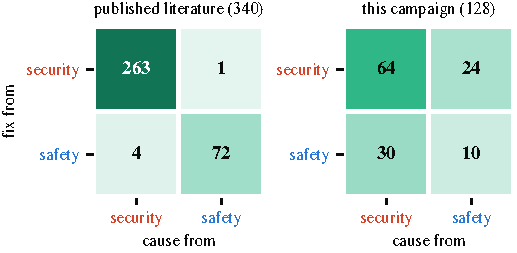
\includegraphics[width=\columnwidth]{figures/fig6_transfer}
\caption{Who built the defense (rows) against whose problem it was run
(columns). Left, every confirmed pair in the literature; right, every pair
in this campaign. Shade is each cell's share of its own panel, so the two
panels are not on one colour scale and the printed count is the value. The
literature crosses between the communities in \NCrossCommunityPairs{} pairs
of \NPureRegimePairs{} (\PctCrossCommunity{}\%); one of its two
off-diagonal boxes holds a single pair. All four boxes are occupied on the
right.}
\label{fig:transfer}
\end{figure}

% GENERATED by scripts/gen_experiment_table.py -- do not hand-edit.
\begin{table}[t]
\centering
\caption{Every kind of run in the campaign, and the question each one was built to settle. Counts are distinct runs of that kind, not scored items.}
\label{tab:experiments}
\small
\begin{tabular}{@{}>{\raggedright\arraybackslash}p{0.62\columnwidth}rl@{}}
\toprule
what the run does & how many & answers \\
\midrule
a defense meets a failure from the other literature, in the retrieval cell & 54 & RQ2 \\
the same, inside a tool-using agent & 56 & RQ2 \\
the same defense against a different shape of planted passage & 10 & RQ3 \\
the same model with no document, and on a second model & 12 & RQ4 \\
two implementations of one defense design & 2 & RQ4 \\
an attack built against the defense it meets & 2 & RQ5 \\
two defenses stacked & 2 & design rule \\
\bottomrule
\end{tabular}
\end{table}


Table~\ref{tab:experiments} lists the kinds of run and the question each one
was built to settle. The first two kinds are the crossings and the home
ground above. The third varies the shape of the planted passage while holding
the defense and the dose fixed, so that a defense which behaves differently
across shapes tells us what it is keying on. The fourth and fifth are
measurements the published evaluations leave out: what the same model scores
with no document at all, and whether a result holds on a second model or on a
second implementation of the same design. The sixth builds the attack against
the defense it meets instead of pointing a fixed attack at it. The last
stacks two defenses that act at different stages.

Every run carries the same arms. A clean arm with nothing planted, an
undefended arm on the same items at the same dose, and a closed-book arm
that sees no document. Every comparison in this paper is a defended arm
against its own undefended arm, never against a number from another run, and
every difference smaller than that run's detectability threshold is reported
as unresolved rather than as zero.

In total we executed \NCampaignPairs{} distinct (defense, attack) pairs
across \NCampaignImpl{} defense implementations, over \NCampaignEpisodes{}
scored episodes: \NRagPairs{} pairs and \NRagEpisodes{} episodes in the
retrieval cell, \NAgentPairs{} pairs and \NAgentEpisodes{} episodes in the
agent cell. An agent episode is a complete multi-step tool-use trajectory and
a retrieval episode is one scored answer, so the two episode counts are not
the same unit.
